%%%%%%%%%%%%%%%%%%%%%%%%%%%%%%%%%%%%%%%%%
% University Assignment Title Page 
% LaTeX Template
% Version 1.0 (27/12/12)
%
% This template has been downloaded from:
% http://www.LaTeXTemplates.com
%
% Original author:
% WikiBooks (http://en.wikibooks.org/wiki/LaTeX/Title_Creation)
%
% License:
% CC BY-NC-SA 3.0 (http://creativecommons.org/licenses/by-nc-sa/3.0/)
% 
% Instructions for using this template:
% This title page is capable of being compiled as is. This is not useful for 
% including it in another document. To do this, you have two options: 
%
% 1) Copy/paste everything between \begin{document} and \end{document} 
% starting at \begin{titlepage} and paste this into another LaTeX file where you 
% want your title page.
% OR
% 2) Remove everything outside the \begin{titlepage} and \end{titlepage} and 
% move this file to the same directory as the LaTeX file you wish to add it to. 
% Then add \input{./title_page_1.tex} to your LaTeX file where you want your
% title page.
%
%%%%%%%%%%%%%%%%%%%%%%%%%%%%%%%%%%%%%%%%%

%----------------------------------------------------------------------------------------
%	PACKAGES AND OTHER DOCUMENT CONFIGURATIONS
%----------------------------------------------------------------------------------------

\documentclass[12pt]{article}
\usepackage[utf8]{inputenc}
\usepackage[french]{babel}
\usepackage[babel=true]{csquotes}
\usepackage{bold-extra}
\usepackage{lmodern,textcomp}


%%%%%%\usepackage{hyperref}
%\usepackage[super,square]{natbib}

%% BIBTEX %%
\usepackage[backend=biber, sorting=none, style=numeric, natbib=true]{biblatex}
\DeclareCiteCommand{\supercite}[\mkbibsuperscript]
  {\iffieldundef{prenote}
     {}
     {\BibliographyWarning{Ignoring prenote argument}}%
   \iffieldundef{postnote}
     {}
     {\BibliographyWarning{Ignoring postnote argument}}}
  {\usebibmacro{citeindex}%
   \bibopenbracket\usebibmacro{cite}\bibclosebracket}
  {\supercitedelim}
  {}
\let\citep=\supercite
%\usepackage[round]{natbib}
%\addbibresource{finite_state_machine.bib}
\bibliography{finite_state_machine}
%%

%% Centrer de grand tableau et figures %%
\usepackage{adjustbox}
\usepackage{array,multirow,makecell,tabularx}
\setcellgapes{1pt}
\makegapedcells
%\newcolumntype{R}[1]{>{\raggedleft\arraybackslash }b{#1}}
%\newcolumntype{L}[1]{>{\raggedright\arraybackslash }b{#1}}
%\newcolumntype{C}[1]{>{\centering\arraybackslash }b{#1}}
\newcolumntype{C}{>{\centering}X}
%%

\usepackage{longtable}
\usepackage{graphicx} 
\usepackage{xifthen}
\usepackage{tabularx}
\usepackage{adjustbox}
\usepackage{amsmath}
%\usepackage[clean,pdf]{svg}
\usepackage{pdfpages}
\usepackage[unicode,hidelinks]{hyperref}
\usepackage[]{url}
%\usepackage{tablefootnote}
\usepackage{footnote}
%\usepackage[bottom]{footmisc}
%\makesavenoteenv{tabular}
\makesavenoteenv{table}
\makesavenoteenv{tabularx}

%\usepackage[super,square]{natbib}

%\newenvironment{agrandirmarges}[2]{%
%\begin{list}{}{%
%\setlength{\topsep}{0pt}%
%\setlength{\listparindent}{\parindent}%
%\setlength{\itemindent}{\parindent}%
%\setlength{\parsep}{0pt plus 1pt}%
%\ifthenelse{\isodd{\value{page}}}%
%{\setlength{\leftmargin}{-#1}\setlength{\rightmargin}{-#2}}
%{\setlength{\leftmargin}{-#2}\setlength{\rightmargin}{-#1}}
%}\item }%
%{\end{list}}



\usepackage[nottoc, notlof, notlot]{tocbibind}

\usepackage[left=4.2cm,right=4.2cm,top=3.5cm,bottom=3.5cm]{geometry}

\newcommand{\doctitle}{Implémentation des Machines à nombre Fini d'États}
\newcommand{\authorName}{Olivier \textsc{Radisson}}
\usepackage{fancyhdr}
\pagestyle{fancy}
\lhead{\doctitle}
\rhead{\authorName}
%\lfoot{Document réalisé par l'équipe n$^\circ$4}
\renewcommand{\headrulewidth}{0.4pt}
\renewcommand{\footrulewidth}{0.4pt}
\renewcommand{\newline}{~\\~\\}
\newcommand{\p}{\newline \indent}
\newcommand{\rt}{~\\ \indent}
\newcommand{\centergraph}[3][]{\begin{center}%
\begin{figure}[h!]%
\vspace{-5pt}%
\centerline{\includegraphics[width=#3]{#2}}%
\ifthenelse{\isempty{#1}}{}{\vspace{-8pt}\caption{#1}}%
\vspace{-5pt}%
\label{#2}%
\end{figure}%
\end{center}}
\newcommand{\newparagraph}{~\\\indent}

\setcounter{secnumdepth}{3}
%\setcounter{tocdepth}{2}


\begin{document}




\begin{titlepage}

\newcommand{\HRule}{\rule{\linewidth}{0.5mm}} % Defines a new command for the horizontal lines, change thickness here

\center % Center everything on the page
 
%----------------------------------------------------------------------------------------
%	HEADING SECTIONS
%----------------------------------------------------------------------------------------

\textsc{\LARGE Institut National des Sciences Appliquées de Lyon\\
\&\vspace{10pt}~
\\KompleXKapharnaüM}\\[1.0cm] % Name of your university/college
\textsc{\small Stage de 4\up{ème} année du département Génie Électrique} \\[0.2cm]
\textsc{\Large Projet Do Not Clean}
\\[0.5cm] % Major heading such as course name
\textsc{\large Réalisation d'une carte multimédia programmable et contrôlable via wifi}\\[0.5cm] % Minor heading such as course title

%----------------------------------------------------------------------------------------
%	TITLE SECTION
%----------------------------------------------------------------------------------------

\HRule \\[0.4cm]
%{ \huge  \textsc{\textbf{Plan Projet}}}\\[0.4cm] % Title of your document
{ \huge   \scshape{\doctitle}  } % \bfseries
\HRule \\[1.5cm]
 
%----------------------------------------------------------------------------------------
%	AUTHOR SECTION
%----------------------------------------------------------------------------------------

\begin{minipage}{0.4\textwidth}
\begin{flushleft} \large
\emph{Auteur:}\\
Olivier \textsc{Radisson}\\
~ \\
~ \\
~ \\
~ \\
\end{flushleft}
\end{minipage}
~
\begin{minipage}{0.4\textwidth}
\begin{flushright} \large
\emph{Tuteur de stage :} \\
Gilles \textsc{Gallet}
~ \\
~ \\
\emph{Chef de projet :} \\
Pierre \textsc{Hoezelle}
~ \\
~ \\

\end{flushright}
\end{minipage}\\[2cm]

% If you don't want a supervisor, uncomment the two lines below and remove the section above
%\Large \emph{Author:}\\
%John \textsc{Smith}\\[3cm] % Your name

%----------------------------------------------------------------------------------------
%	DATE SECTION
%----------------------------------------------------------------------------------------
\vspace{2.2cm}
{\large - 6 octobre 2014 -}\\ \vspace{10pt}
{\large Dernière édition le \today}\\
%{\large  ~~~ : \today}\\[3cm] % Date, change the \today to a set date if you want to be precise

%----------------------------------------------------------------------------------------
%	LOGO SECTION
%----------------------------------------------------------------------------------------

%\includegraphics{Logo}\\[1cm] % Include a department/university logo - this will require the graphicx package
 
%----------------------------------------------------------------------------------------

\vfill % Fill the rest of the page with whitespace

\end{titlepage}


%\newpage
%~
%	\thispagestyle{empty}
    

\newpage
\thispagestyle{empty}
\begin{abstract}
Ce document présente l'implémentation qui est faite des Machines à nombre fini d'États\footnote{De l'anglais \textit{Finite State Machine} traduit communément de façon maladroite par Machina à États Finis}. Cette implémentation n'est pas rigoureuse d'un point de vue mathématique mais étend son application habituelle aux problématiques rencontrées sur le projet.\p
Une FSM est toujours dans un état définit auparavant et possède pour chaque état un nombre fini de transitions qui seront franchies dès que leur condition sera validée. Une fois une transition franchie la FSM change d'état et attends de nouveau qu'une transition soit franchie.\p
Cette implémentation sert principalement à mettre en place les protocoles nécessaires au fonctionnement de notre réseau et ajoute une grand robustesse à ce niveau. De plus les FSM, comme nous les appellerons désormais dans ce document, serviront de base pour l'implémentation de la logique de scénario.
\p

\end{abstract}

\newpage
~ \thispagestyle{empty}
%\newpage
%\thispagestyle{empty}

\tableofcontents

%\newpage
%~ \thispagestyle{empty}
\newpage

\setcounter{page}{1}

\section{Introduction}
\textit{Ce document à une visée majoritairement technique. Les points abordés peuvent intéresser les utilisateurs les plus curieux, mais sa vocation première est de présenter l'implémentation faite d'une certaine logique d'automatisme pour documenter le développement du projet.}\p
La partie logique du projet doit gérer de nombreuses chose comme des protocoles de synchronisation du temps ou l'exécution de scénarios définis à l'avance. Ces comportements se doivent d'être le plus sûr possible, c'est à dire résistants aux imprévus comme la connexion simultanée de plusieurs cartes sur le réseau ou l'attente d'un message qui s'est perdu en route.\p
Pour répondre à cet objectif, le projet se basera sur une implémentation de la logique des Machines à nombre fini d'Étapes\footnote{De l'anglais \textit{Finite State Machine} traduit communément de façon maladroite par Machina à États Finis}\citep{encyclopediaArticle_Automatefini_} qui sera adapté aux problématiques rencontrées.\p
Tout au long de ce document sera utilisé l'acronyme FSM pour \textit{Finite State Machine}, origine anglophone du terme Machine à nombre fini d'États.

\section{Présentation succincte des FSM}
Une FSM peut être représentée par un graphique comme celui-ci :
\begin{figure}[htbp]
  \centering
  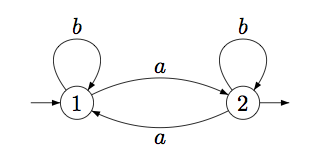
\includegraphics[width=0.55\textwidth]{figs/Automate-impair.png}
  \caption{Exemple de FSM}
  \label{fig:fsm_example}
  %\vspace{-17pt}
\end{figure}~\\
Ici la machine présentée possède deux états 1 et 2 ainsi que deux signaux $a$ et $b$. Si la FSM est à l'état 1 et reçois le signal $a$ celle-ci passera dans l'état 2.\p
Une machine possède un nombre fini d'états, ici 2 en l'occurrence. Un certain nombre de signaux, ici $a$ et $b$. Et à chaque état est associé aucun, un ou plusieurs signaux qui peuvent permettre à la machine de changer d'état.

\section{Implémentation des FSM dans le projet}
La différence principale entre les FSM théorique et celle qui seront utilisées dans le projet provient des signaux qui sont plus complexe que de simple valeur.\p
De plus il existe des étapes conditionnelles qui ne sont pas des états pour la machine mais qui permet de traiter un signal pour activer, ou non, une transition.

\subsection{Les signaux}
Tout d'abord il faut définir deux notions qui sont ajoutées ici : 
\begin{itemize}
\item \textbf{JTL}\footnote{\textit{Jump To Live}} : Le nombre de saut avant la mort du signal
\item \textbf{TTL}\footnote{\textit{Time To Live}} : Le temps de vie d'un signal
\end{itemize}~\\
\indent Ces notions permettent au signaux de ne pas être ignorés directement si ils ne correspondent pas à une transition. Ils sont placé en mémoire dans une pile et pourront déclencher des transitions tant que aucun de ses paramètres \textbf{TTL} et \textbf{JTL} ne sont pas expirées.\p
De plus les signaux peuvent transporter un certain nombre d'arguments tel que les valeurs reçus dans un message OSC, ou le résultat d'une opération précédente.\\
Enfin chaque message peut se voir attribuer une action lorsque celui-ci est ignoré.

\begin{table}[htbp]
\centering

\textbf{Signal}\vspace{8pt}~\\

\begin{tabularx}{0.95\textwidth}{|c|c|c|C|c|}
\hline
\textbf{ID} & \textbf{JTL} & \textbf{TTL} & \textbf{Arguments} & \textbf{Ignoré}  \tabularnewline
\hline
\hline
RECV\_MSG & 1 & 0.5 & (/iamhere, name, \textit{timetag}) & - \tabularnewline
\hline
\end{tabularx}
\vspace{10pt} 
\label{tab:sig_exemple}
\caption{Exemple d'un signal pour le réception d'un message OSC}
%\vspace{-25pt}
\end{table}

\subsection{Les états}
Les états sont la base de la logique d'une FSM. Chaque à un identifiant unique, par exemple, \textit{MAIN\_WAIT} qui peut être l'état principal d'attente pour un protocole. De plus chaque état à une fonction qui lui est attribuée et qui est lancé lorsque la machine change d'état.\p
De plus chaque état à un verrou de préemptibilité permettant d'indiquer si l'action de l'étape est bien terminée et si la FSM peut en changer si un signal lui indique.\p
Enfin chaque état possède un certain nombre de transitions qui lui sont associées.

\begin{table}[htbp]
\centering

\textbf{État}\vspace{8pt}~\\

\begin{tabularx}{0.95\textwidth}{|c|c|C|c|}
\hline
\textbf{ID} & \textbf{Action} & \textbf{Transition} & \textbf{Préemptible}  \tabularnewline
\hline
\hline
MAIN\_WAIT & \textit{\_pass} & RECV\_MSG: step\_iamhere & True \tabularnewline
\hline
\end{tabularx}
\vspace{10pt} 
\label{tab:sig_exemple}
\caption{Exemple d'état : Attente de message d'un protocole}
%\vspace{-25pt}
\end{table}

\subsection{Les transitions et conditions}

Les transitions sont de simples listes de doublet entre un signal et, soit un autre état, soit une condition.\p
Les conditions sont de simples fonctions qui prennent en paramètre le signal les ayant déclenchées et retournant, soit un état vers le quel transité, soit une valeur nulle pour signifier que le signal ne doit pas déclencher de changement d'état.

\section{Exemple d'application d'une FSM}
Cet exemple est une partie de la FSM qui gère le protocole de synchronisation dans le réseau. L'exemple concerne la partie synchronisation du temps côté référence.
\subsection{Principe du protocole à implémenter}
Depuis l'état principal d'attente, si la FSM reçoit un message OSC $/rtp/asktime$ celle-ci va démarrer une synchronisation en envoyant une série de \textbf{ping} et attendant pour chaqu'un d'eux une réponse \textbf{pong} correspondante. Pour chaque échange il va chercher le temps de trajet et tenter, avec un échantillon assez représentatif\footnote{La procédure exacte n'est pas traité ici car ce n'est pas le sujet principal}, d'identifier le temps de parcours moyen pour ensuite envoyer son temps plus le correctif à appliquer.
\subsection{États}
Les états de fonctionnements sont les suivants :\\
\begin{itemize}
\item \textbf{MAIN\_WAIT} : État d'attente principale du protocole.
\item \textbf{START\_SYNC} : État initialisant les variables nécessaires à la synchronisation et un timer pour éviter de rester bloquer lors de la synchronisation.
\item \textbf{SEND\_PING} : État envoyant un \textbf{ping} et notant la date d'envoi dans une variable.
\item \textbf{WAIT\_PONG} : État d'attente après l'envoie d'un \textbf{ping}
\item \textbf{RECV\_PONG} : État de réception d'un \textbf{pong} et de calcul du temps de parcours puis de l'éventuelle synchronisation
\item \textbf{SEND\_SYNC} : État envoyant un message de synchronisation 
\end{itemize}

\subsection{Conditions}
Dans ce fonctionnement il y a une transition conditionnelle qui se situe après la réception d'un \textbf{pong}. Si les valeurs de temps de parcours sont cohérentes et que la synchronisation est possible cette condition renvoie vers l'état \textbf{SEND\_SYNC} sinon elle retourne l'état \textbf{SEND\_PING} pour que cela continue.

\subsection{Signaux}
Les principaux signaux sont les suivants :~\\
\begin{table}[htbp]
\vspace{-5pt}
\centering

\textbf{Signaux}\vspace{8pt}~\\

\begin{tabularx}{0.95\textwidth}{|c|c|c|C|c|}
\hline
\textbf{ID} & \textbf{JTL} & \textbf{TTL} & \textbf{Arguments} & \textbf{Ignoré}  \tabularnewline
\hline
\hline
RECV\_MSG & 1 & 0.5 & (/rtp/asktime, ...) & - \tabularnewline
\hline
RECV\_MSG & 1 & - & (/rtp/pong, ...) & - \tabularnewline
\hline
TIME\_OUT & 3 & - & - & - \tabularnewline
\hline
\end{tabularx}
\vspace{10pt} 
\label{tab:sig_exemple}
\caption{Signaux présents dans l'exemple}
%\vspace{-25pt}
\end{table}

On peut voir ici qu'il y a deux signaux avec le même identifiant. En réalité une petit fonction permet de créer facilement et de manière transparente des conditions lors de la réception d'un message OSC en fonction de l'adresse de celui-ci. Un signal \textbf{RECV\_MSG} ne déclenchera la passage à \textbf{START\_SYNC} que si son adresse est \textit{/rtp/asktime}.

\subsection{Implémentation du protocole}
\begin{figure}[htbp]
  \centering
  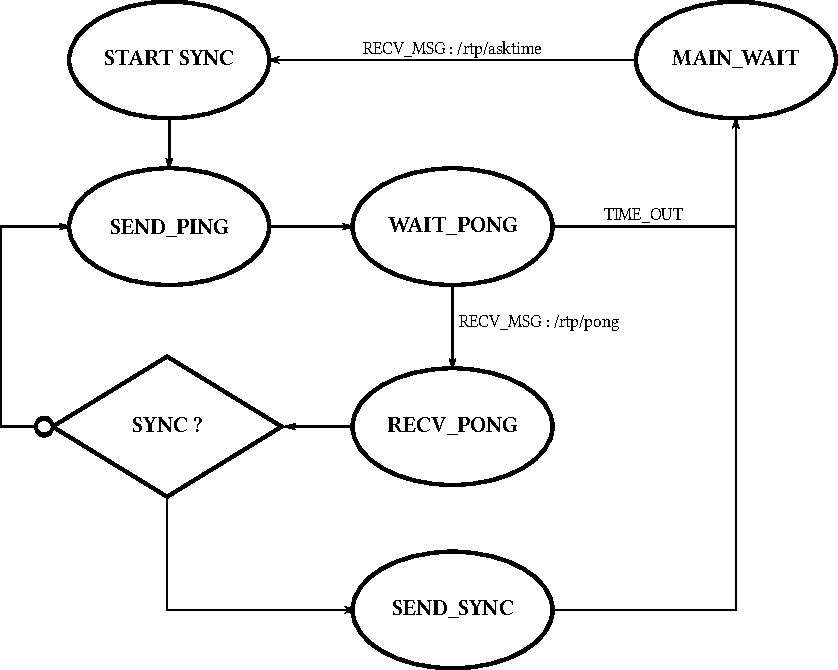
\includegraphics[width=0.95\textwidth]{figs/exemple_fsm.pdf}
  \caption{Implémentation du protocole avec une FSM}
  \label{fig:fsm_sync}
  \vspace{-17pt}
\end{figure}~\\

Les transitions représentées par une flèche sans signal sont des transitions directes, franchies dès que l'état est préemptible.\p
   
   
%\newpage
%\section{Annexes}
%	\subsection{Bibliographie}
% \def\refname{}%
\nocite{webpage_FiniteStateAutomata_}
%\bibliographystyle{plain-url}
%\bibliography{finite_state_machine}
\printbibliography
%\newpage\textsc{•}


\end{document}